% 导言区
  \documentclass{ctexart}%ctexbook, ctexrep
  \usepackage{graphicx}	
  \graphicspath{figures/}
  %\usepackage{ctex}
  % 正文区(文稿区)
  \begin{document}
  	电脑壁纸见图\ref{fig-wallpaper}% 实现交叉引用
  	\begin{figure}[htbp]%图形位置 h 当前位置 t 顶部 b 底部 p 浮动页
  		\centering % 居中排列
  		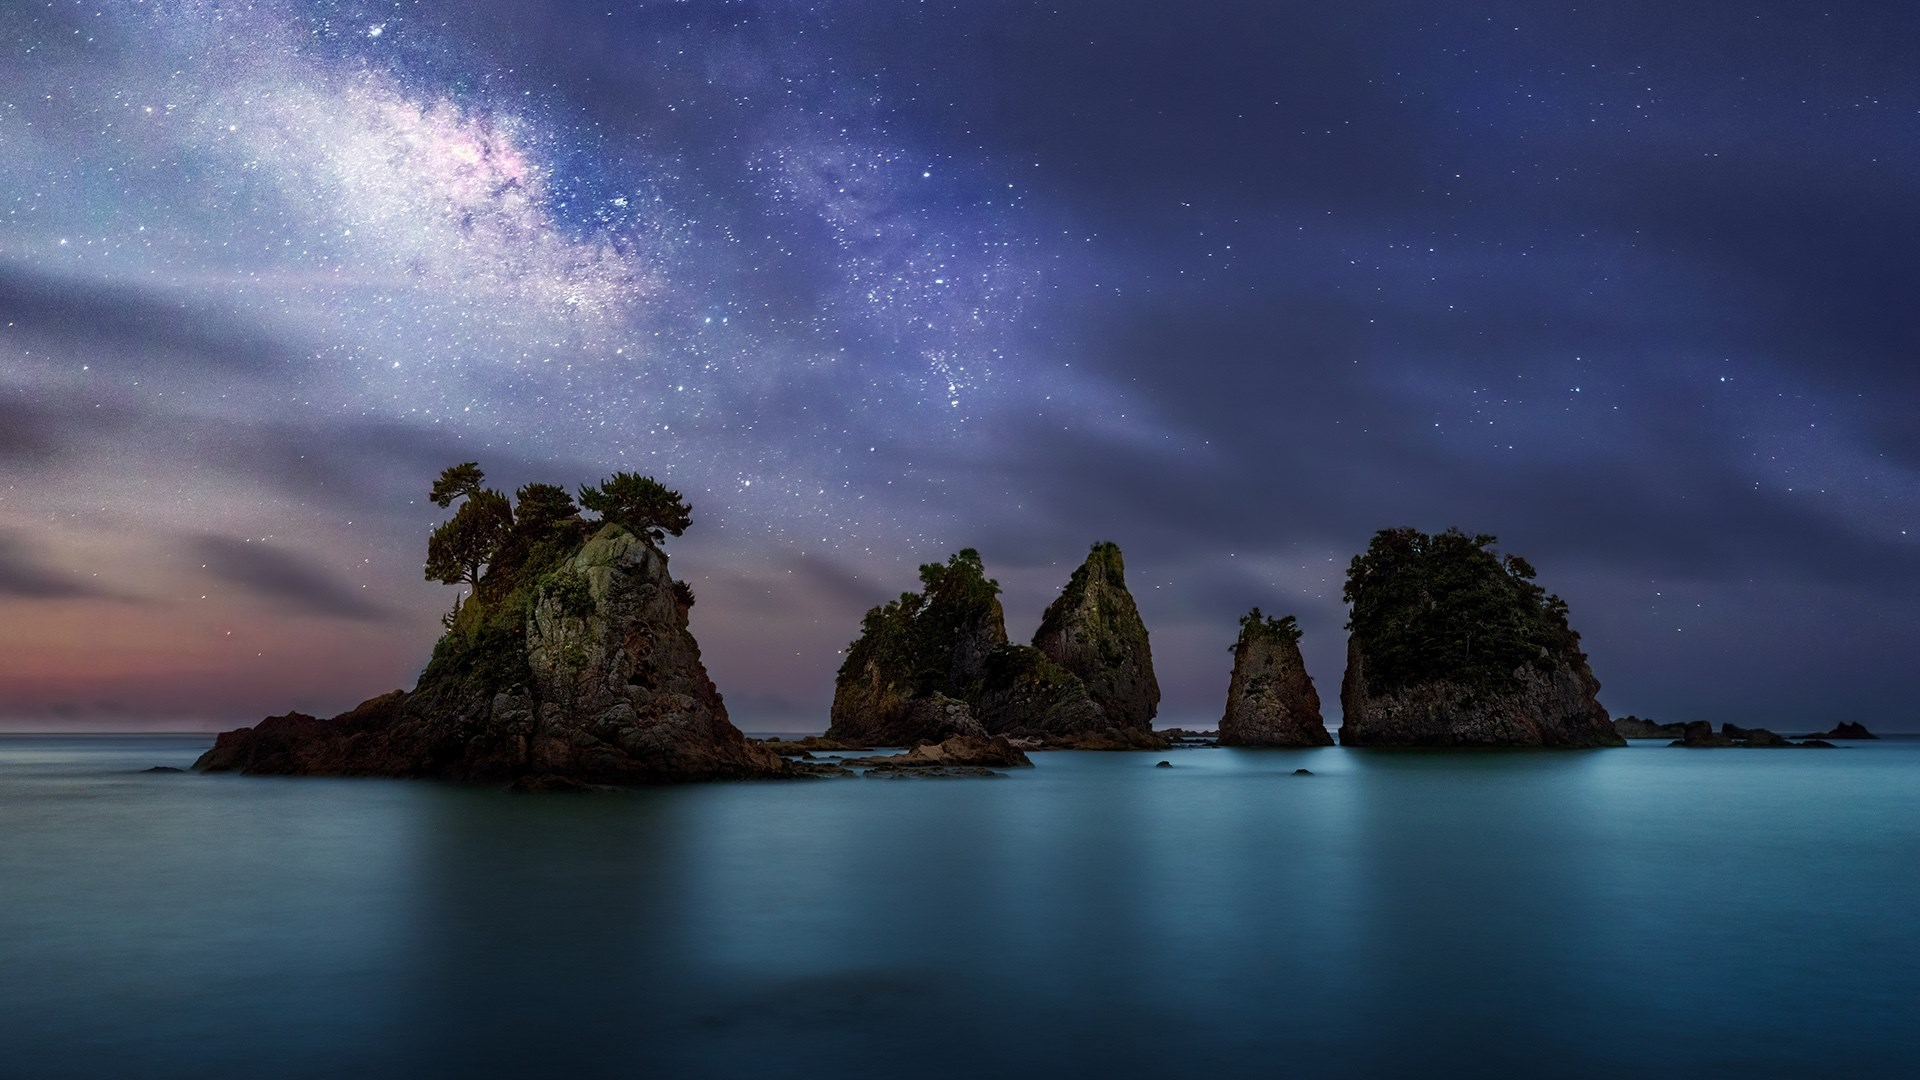
\includegraphics[scale=0.25]{wallpaper}% 输入图片名,指定缩放因子
  		\caption{WallPaper}\label{fig-wallpaper} %设置图片名字 设置浮动体标签
  	\end{figure}
  	
  	当然,在\LaTeX{}中也如以下使用表\ref{tab-score}所示的表格
  	\begin{table}[h]
  		\centering
  		\caption{考试成绩单}\label{tab-score}
  		\begin{tabular}{|l|c|c|c|r|}
  			\hline %产生横线
  			姓名 & 语文 & 数学 & 外语 & 备注 \\
  			\hline %产生横线
  			张三 & 87 & 100 & 93 & 优秀 \\
  			\hline %产生横线
  			李四 & 75 & 64 & 52 & 补考另行通知 \\
  			\hline %产生横线
  			王二 & 80 & 82 & 78 & \\ 
  			\hline %产生横线	
  		\end{tabular}
  	\end{table}
  	
\end{document}